\documentclass[11pt, logo, nonumbering]{preprint}
\usepackage[utf8]{inputenc}
\usepackage{microtype}
\usepackage{graphicx}
%\usepackage{times}
\usepackage{amsmath}
\usepackage{booktabs}
\usepackage{enumitem}
\usepackage{xcolor}
\definecolor{mydarkblue}{rgb}{0,0.08,0.45}
\usepackage[colorlinks=true,linkcolor=mydarkblue,citecolor=mydarkblue,filecolor=mydarkblue,urlcolor=mydarkblue]{hyperref}
\usepackage{xspace}
\usepackage{cleveref}
\usepackage{tikz}
\usetikzlibrary{arrows.meta}

% Bibliography machinery retained for later use; this proposal cites sources as
% inline hyperlinks, so no bibliography is printed.
\IfFileExists{csquotes.sty}{\usepackage{csquotes}}{}
\IfFileExists{biblatex.sty}{%
  \usepackage[style=numeric-comp,natbib=true,maxbibnames=3,minnames=1,backend=bibtex,doi=false,eprint=false,url=false]{biblatex}
  \addbibresource{ref.bib}
}{%
  \usepackage[numbers,sort&compress]{natbib}
}

% Custom colors for your paper
\definecolor{gred}{RGB}{250, 210, 207}
\definecolor{coolblue1}{rgb}{0.91, 0.94, 0.98}
\definecolor{coolblue2}{rgb}{0.76, 0.85, 0.94}
\definecolor{coolblue3}{rgb}{0.54, 0.72, 0.87}
\definecolor{coolblue4}{rgb}{1, 1, 1}

% Custom commands for your paper
\newcommand{\ourbench}{\textsc{YourBenchmark}\xspace}
\newcommand{\ourbenchmini}{\texttt{YourBenchmark-mini}\xspace}
\newcommand{\ourbenchnum}{XXX\xspace}
\newcommand{\ourmodel}{YourModel\xspace}
\newcommand{\ourbaseline}{YourBaseline\xspace}






% for tableofcontent
% \usepackage{tocloft}
% \renewcommand{\contentsname}{\hfill\bfseries\Large Contents\hfill}   
% \renewcommand{\cftaftertoctitle}{\hfill}
% \renewcommand{\listtablename}{\hfill\bfseries\Large List of Tables} % no \hfill after "List of Tables"...
%%% using the command "\renewcommand{\cftlottitlefont}{\hfill\bfseries\Large}" works too...
% \renewcommand{\cftafterlottitle}{\hfill}


% Custom styling (add your own as needed)


\newcommand{\method}{}


\begin{document}

\title{Targeted de novo nanobody design through backbone generation and sequence optimization} 
 

\author{
\textbf{Aidan Jan}$^{1}$ \quad
\textbf{Charlie Yang}$^{1}$ \quad
\textbf{Jeffery Wang}$^{1}$ \\
\textsuperscript{1}Carnegie Mellon University\\
\texttt{\{ajan, qiyuy, jdw2\}@andrew.cmu.edu} \\
}

\maketitle


\begin{abstract}
We propose a computational study of nanobody design for a specified protein epitope. The pipeline combines antibody-adapted RFdiffusion for backbone generation, ProteinMPNN for sequence design, and structure prediction with Alphafold 3 scoring for candidate selection. We will test how epitope constraints, sequence sampling, and filtering affect design quality and diversity. The intended outcome is a reproducible workflow and a shortlist of candidates for experimental testing.

\end{abstract}

\section{Introduction}
\label{sec:intro}
Nanobodies are compact antibody fragments that can recognize specific protein surfaces. Designing them against a chosen epitope could support targeted therapeutics and molecular detection. The central problem is to identify sequences that both retain the nanobody fold and form the intended binding interface.\\\\
Sequence generation alone does not explicitly establish a binding geometry. Conversely, a plausible backbone may lack a sequence that reliably adopts it. Existing structure-based methods address these problems, but candidate selection remains uncertain: prediction confidence measures structural confidence, not experimental binding success. \href{https://www.ebi.ac.uk/training/online/courses/alphafold/inputs-and-outputs/evaluating-alphafolds-predicted-structures-using-confidence-scores/confidence-scores-in-alphafold-multimer/}{AlphaFold confidence documentation}\\\\
We propose to implement and evaluate an epitope-directed design pipeline built on existing models. The intuition is to constrain the binding geometry first, sample compatible sequences, and then check whether predicted structures recover the intended interface. The research contribution will be a controlled evaluation of design and selection choices within this established approach.


\section{Related Work}
\label{sec:related}
\begin{center}
\small
\begin{tabular}{@{}p{0.23\linewidth} p{0.71\linewidth}@{}}
\toprule
\textbf{Category} & \textbf{Relevant work and relationship to this project} \\
\midrule
Backbone generation & \href{https://www.nature.com/articles/s41586-023-06415-8}{RFdiffusion} generates protein backbones under structural constraints. It provides the basis for target-conditioned design. \\
\addlinespace
Antibody-specific design & \href{https://github.com/RosettaCommons/RFantibody}{RFantibody} already combines antibody-adapted RFdiffusion, ProteinMPNN, and antibody-adapted RoseTTAFold2. This is the closest precedent and the starting point for our evaluation. \\
\addlinespace
Inverse folding & \href{https://github.com/dauparas/ProteinMPNN}{ProteinMPNN} designs sequences conditioned on backbone structure. We will examine how sequence sampling affects candidate diversity and structural recovery. \\
\addlinespace
Computational assessment & AlphaFold confidence metrics and \href{https://docs.rosettacommons.org/docs/latest/application_documentation/analysis/interface-analyzer}{Rosetta InterfaceAnalyzer} provide complementary structural and interface assessments. We will evaluate their usefulness for ranking candidates. \\
\bottomrule
\end{tabular}
\end{center}

\subsection{Existing Methods and Availability}
\begin{itemize}
    \item \textbf{BoltzGen:} a broader binder-design framework with nanobody support. Public code and weights; a possible comparison method. \url{https://github.com/HannesStark/boltzgen}
    \item \textbf{DiffAb:} joint antibody sequence and structure design. Public code and weights; useful for CDR redesign comparisons, although its input assumptions differ.
    \url{https://github.com/luost26/diffab}
\end{itemize}


\section{Proposed Method}
\label{sec:method}
% \begin{figure}[htbp]
% \centering
% \includegraphics[width=0.33\linewidth]{fig/pipeline.png}
% \end{figure}

\begin{center}
    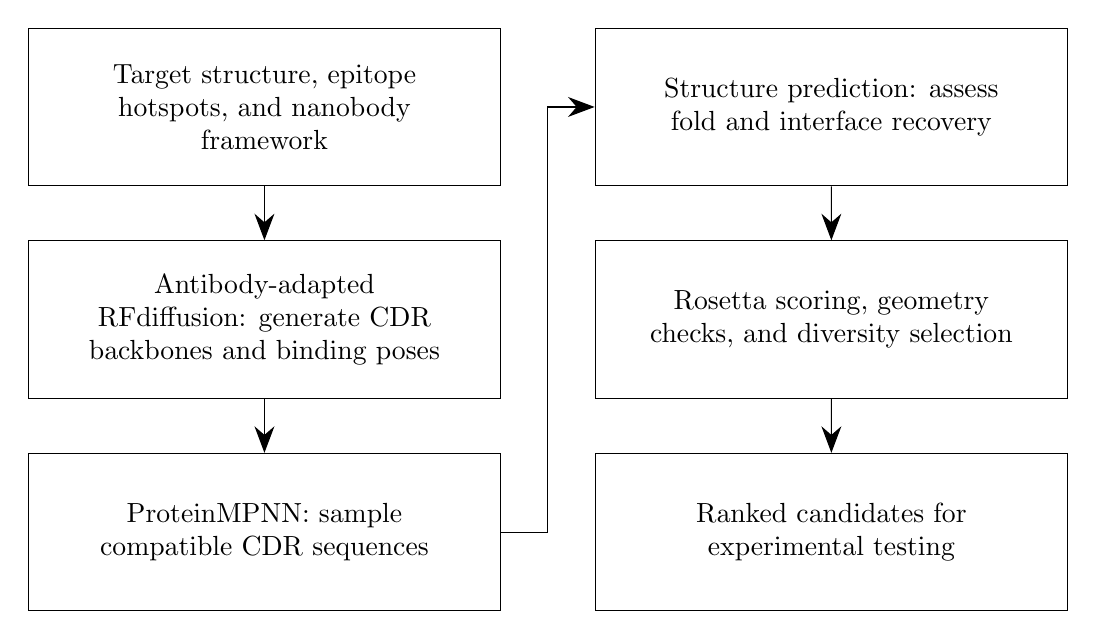
\begin{tikzpicture}[scale=0.9]
        \node[draw, align=center, minimum height=2cm, minimum width=6cm] at (0, 0) (a) {Target structure, epitope \\ hotspots, and nanobody \\ framework};
        \node[draw, align=center, minimum height=2cm, minimum width=6cm] at (0, -3) (b) {Antibody-adapted \\ RFdiffusion: generate CDR \\ backbones and binding poses};
        \node[draw, align=center, minimum height=2cm, minimum width=6cm] at (0, -6) (c) {ProteinMPNN: sample \\ compatible CDR sequences};
        \node[draw, align=center, minimum height=2cm, minimum width=6cm] at (8, 0) (d) {Structure prediction: assess \\ fold and interface recovery};
        \node[draw, align=center, minimum height=2cm, minimum width=6cm] at (8, -3) (e) {Rosetta scoring, geometry \\ checks, and diversity selection};
        \node[draw, align=center, minimum height=2cm, minimum width=6cm] at (8, -6) (f) {Ranked candidates for \\ experimental testing};

        \draw[-{Stealth[scale=2]}] (a) -- (b);
        \draw[-{Stealth[scale=2]}] (b) -- (c);
        \draw[-{Stealth[scale=2]}] (c.east) -| (4, 0) -- (d);
        \draw[-{Stealth[scale=2]}] (d) -- (e);
        \draw[-{Stealth[scale=2]}] (e) -- (f);
    \end{tikzpicture}
\end{center}
We will preserve a selected nanobody framework while generating its complementarity-determining regions (CDRs) around the specified target surface. ProteinMPNN will sample multiple CDR sequences for each backbone while keeping the framework sequence fixed.\\\\
Then, we will predict complexes without supplying the generated CDR backbone or binding pose as a template. Evaluation will include framework and CDR pLDDT, interchain PAE, ipTM where available, hotspot contacts, and deviation from the designed interface after target alignment.\\\\
Rosetta interface scores and shape complementarity will help rank geometrically plausible candidates. These scores are approximate computational assessments, not measured binding free energies. Selection thresholds will be calibrated on a development set before evaluation on held-out targets.


\section{Experiments}
\label{sec:experiment}
We will evaluate three aspects of the pipeline: recognition of known binders,
ranking by measured affinity, and generation of new candidates against targets
with known nanobody complexes. The first two experiments assess candidate
selection using experimental labels; the third assesses computational design
quality. Comparisons will use matched computational budgets and repeated random
seeds where applicable. The claims below are hypotheses to test.

\begin{center}
\small
\begin{tabular}{@{}p{0.26\linewidth} p{0.35\linewidth} p{0.31\linewidth}@{}}
\toprule
\textbf{Research question} & \textbf{Proposed claim} & \textbf{Evidence needed} \\
\midrule
Can our filter recognize known binders?
& Combining structural confidence, interface geometry, and Rosetta scores
ranks experimentally labeled binders above nonbinders more effectively than
confidence alone.
& Precision-recall curves; precision among top-ranked candidates; comparison
of individual and combined filters on AVIDa datasets. \\
\addlinespace
Can our scores distinguish stronger from weaker binders?
& Combined scores better reproduce measured affinity rankings than individual
scores for nanobodies tested against the same target under comparable
assay conditions.
& Spearman correlations; predicted-score versus measured-$pK_D$ plots;
recovery of the strongest measured binders. \\
\addlinespace
Can we generate plausible alternatives for targets with known complexes?
& Hotspot conditioning increases the yield of distinct candidates that retain
intended epitope contacts after reprediction compared with unguided generation
at matched computational cost.
& Per-target computational pass rates; contact recovery; CDR RMSD;
interface overlays; distinct candidate yield versus GPU-hours. \\
\bottomrule
\end{tabular}
\end{center}

\paragraph{Binding labels.}
For binding classification, we will use nanobody sequences and experimental binding/nonbinding labels from AVIDa-hIL6, with AVIDa-SARS-CoV-2 as an additional benchmark. These labels reflect screening outcomes rather than quantitative affinity.

\paragraph{Affinity data.}
For affinity ranking, we will curate experimentally measured $K_D$ values from ANDD, SAbDab-nano, and sdAb-DB, exclude predicted affinities, and retain traceable measurement sources. Comparisons will be grouped by target construct and assay where possible. Stronger binding corresponds to lower $K_D$, or higher $pK_D = -\log_{10}(K_D/\mathrm{M})$.

\paragraph{Generation targets.}
Design targets are drawn from the SAbDab2 machine learning dataset \href{https://zenodo.org/records/22019991}{(v0.2.0)}, using the single-domain antigen-aware split (\texttt{abag\_split\_sd.csv}), in which antibodies are clustered by CDR sequence identity and protein antigens at 40\% identity, so that no antigen family appears in both partitions. Restricting to single-domain heavy-chain entries bound to a protein antigen yields 1{,}578 structures across 941 PDB entries, partitioned into 143 training clusters and 43 held-out test clusters. Because this split controls sequence redundancy but not structure recency, held-out targets are further filtered by PDB deposition date to postdate the training cutoffs of the generative and structure-prediction models used; a 2023 cutoff retains 21 independent test clusters, and cutoffs between 2022 and 2024 vary this count by at most five. Cluster sizes are highly uneven, with the largest test cluster accounting for 22\% of its structures, so a single representative structure per cluster is selected by resolution and each target is weighted equally in all comparisons. The generator will receive the target structure and a predefined epitope, while the reference nanobody's CDR sequences, coordinates, and binding pose remain withheld.

\paragraph{Data separation.}
Development data will be used to select scores and calibrate thresholds; held-out test data will be evaluated only after these choices are fixed. Nanobody sequence and CDR clusters will remain within a single split. Experiments testing generalization across targets will also separate antigen families. Structural benchmarks will use structures deposited after documented model training cutoffs where feasible and will be screened for homologous training examples. A recent deposition date alone does not establish that a target is unseen.

\paragraph{Success criteria.}
Classification and affinity-ranking performance will be assessed against experimental labels. A generated candidate will count as an \emph{in silico} success only if it meets thresholds fixed on the development set for design-to-reprediction CDR backbone RMSD, intended hotspot-contact recovery, interface confidence, and steric clashes. Confidence measures will include interchain PAE, CDR pLDDT, and ipTM where available. Final computational assessment will use a predictor excluded from generation and candidate selection.\\\\
Native-pose metrics such as DockQ will be used only when reconstructing known complexes. Newly generated sequences may adopt valid binding poses that differ from the reference, so similarity to the reference pose will not be required for computational success.

\paragraph{Controls and ablations.}
Candidate-selection experiments will compare confidence-only, geometry-only, energy-only, and combined scoring. Generation experiments will compare hotspot-conditioned and unguided sampling under matched computational budgets. Scrambled CDR sequences may provide supplementary stress tests, but neither scrambled sequences nor untested nanobody--target pairs will be treated as experimentally confirmed nonbinders.

\paragraph{Statistical treatment and compute accounting.}
We will report per-target results and uncertainty estimates that account for sequence relatedness. For AVIDa-hIL6, bootstrap sampling will operate over nanobody clusters, keeping measurements across IL-6 variants together. Multi-target comparisons will use target-level summaries and bootstrap intervals. Generation runs will use a fixed number of random seeds, with designs grouped by backbone and target rather than treated as independent observations. Candidate yield will be plotted against GPU-hours, and distinctness will be defined using prespecified sequence-identity thresholds and CDR structural clustering criteria.

\noindent These experiments will test whether the pipeline identifies measured binders and produces structurally plausible new candidates. Claims that newly generated nanobodies bind, or outperform measured references, will require experimental measurements on those sequences.

\section{Analysis}
\label{sec:analysis}
Ablations will remove hotspot guidance and individual filtering components, and vary sequence sampling depth. Error analysis will distinguish framework distortion, CDR refolding, incorrect binding poses, and steric clashes. We will examine whether failures cluster by target or loop length and report uncertainty across targets and random seeds. Candidate counts will be grouped by backbone to avoid treating closely related sequences as independent evidence.


\section{Conclusion}
\label{sec:conclusion}
We aim to establish which design constraints and screening criteria produce diverse nanobody candidates that consistently recover an intended interface. The project will deliver a reproducible benchmark, an assessment of computational filtering limits, and a shortlist for experimental binding and specificity measurements.


\section{Additional Details}
\label{sec:additional}
\subsection{Directions for Going Forward}
We can develop a candidate-ranking strategy that likely combines structural confidence and inference of geometry, calibrated according to available measured binding data. We can test hotspot guidance from the pipeline and whether, in a computational budget constraint, it is better spent possibly generating more backbones or more sequences per backbone. 

% Three extensions follow naturally from the planned experiments. First, if combined scoring improves ranking on measured binders, the resulting filter can be applied prospectively to the generated candidates to produce a prioritised shortlist, which is the form in which designs would enter an experimental campaign. Second, the filtering comparison can be repeated on binder classes other than nanobodies, testing whether a ranking function calibrated on one design modality transfers to another; existing meta-analyses of de novo binder design are dominated by mini-binders rather than CDR-loop binders, so this transfer is untested. Third, the generation stage currently conditions on a fixed epitope; conditioning instead on a desired specificity profile, for example requiring contacts on one epitope while avoiding a homologous surface, would address cross-reactivity, which is the failure mode most likely to matter for therapeutic use. Experimental validation of a small number of selected candidates by binding assay remains the decisive next step and is outside the scope of this project.

\subsection{Workload Split}
The team consists of three members, and the division follows the three experiments so that work can proceed in parallel once the shared data layer is in place.

\begin{itemize}[nosep]
    \item \textbf{Data and benchmarks.} Curation of AVIDa binding labels and $K_D$ records, construction of the SAbDab2 target set and splits, deposition date filtering, and the evaluation harness. Owns the classification and affinity-ranking experiments.
    \item \textbf{Generation.} Installation and operation of RFantibody and ProteinMPNN, hotspot specification, sampling-depth sweeps, and job orchestration including failure recovery and run manifests. Owns the generation experiment.
    \item \textbf{Evaluation and scoring.} Structure prediction, Rosetta interface scoring, metric implementation, threshold calibration on the development set, and the reward-hacking and leakage diagnostics.
    \item \textbf{All members.} Ablations, error analysis, and the written report.
\end{itemize}

\noindent The first two weeks are shared and sequential, because the outcome of the installation and data audits determines the scope available to each member.  A deliberately simple scoring wrapper will be fixed by the end of week two so that the generation and evaluation work can proceed against a stable interface while the full scoring stack is completed.

\subsection{Timeline}
\begin{center}
\small
\begin{tabular}{@{}c p{0.45\linewidth} p{0.35\linewidth}@{}}
\toprule
\textbf{Date} & \textbf{Work} & \textbf{Gate} \\
\midrule
Oct. 11 & Environment setup; RFantibody and ProteinMPNN installation; structure predictor access & Pipeline runs end to end on one target \\
\addlinespace
Oct. 18 & SAbDab2 target set, date filtering, cluster representatives; AVIDa and $K_D$ curation & Benchmark frozen; split files released \\
\addlinespace
Oct. 25 & Classification and affinity-ranking experiments on development data; threshold calibration & Filter comparison complete on development set \\
\addlinespace
Nov. 1 & Generation on a pilot subset of targets; hotspot versus unguided & \textbf{Midterm report} \\
\addlinespace
Nov. 8 & Full generation sweep across held-out targets and seeds & Per-target yields and contact recovery \\
\addlinespace
Nov. 15 & Sampling-depth sweep; candidate yield versus GPU-hours & Diminishing-returns curve \\
\addlinespace
Nov. 22 & Ablations; error analysis; leakage checks & All controls reported \\
\addlinespace
Nov. 29 & Final analysis, packaging, shortlist assembly & \textbf{Final report} \\
\bottomrule
\end{tabular}
\end{center}


\subsection{Computational Requirements}
Cost is dominated by structure prediction and by the generation sweep rather
than by model training; no component is trained from scratch. Evaluation is
staged: all candidates are screened with the fast predictor bundled with the
design pipeline, and only those passing screening thresholds are re-evaluated
with the higher-accuracy predictor reserved for final scoring, which is excluded
from generation and candidate selection.

\noindent We are requesting approximately 100 GPU-hours and 50 CPU-hours.  Per-run cost depends strongly on antigen size and on predictor configuration, so these figures are derived from the design matrix above combined with assumed per-unit timings; we will measure the end-to-end cost of a single target in week one and rescale the request from that measurement rather than from published timings. We expect the bulk of GPU-hour being budgeted for evaluations, backbone \& sequence generation, and validation of generated candidates. The sampling-depth sweep is the schedule-elastic component: a coarser grid still yields the yield-versus-compute curve that the third research question requires. Storage is modest, under 200\,GB including structure files, predicted complexes with their confidence matrices, and run manifests. At this job count failures are routine rather than exceptional, so the pipeline is built with idempotent re-runs, caching keyed by configuration fingerprint, and per-run resource accounting; these are deliverable features rather than operational conveniences. Access to the final-scoring predictor is the main scheduling dependency and will be confirmed in week one.

% https://genaibiomed.github.io/GenAIBioMed2026Fall/docs/Projects/

\end{document}